% Source: Code/ML_overlay/ir_rgb_registration/paper/ml_overlay_report_materials/ir_rgb_registration_report/figures/fig_pwcnet_architecture.tex
\documentclass[tikz,border=10pt]{standalone}
\usepackage{tikz}
\usetikzlibrary{positioning,shapes.geometric,arrows.meta,calc}

\definecolor{Garnet}{RGB}{115,0,10}
\definecolor{Rose}{RGB}{204,46,64}
\definecolor{Atlantic}{RGB}{70,106,159}
\definecolor{Congaree}{RGB}{31,65,77}
\definecolor{Horseshoe}{RGB}{101,120,11}
\definecolor{Black90}{RGB}{54,54,54}
\definecolor{Black70}{RGB}{92,92,92}

\begin{document}
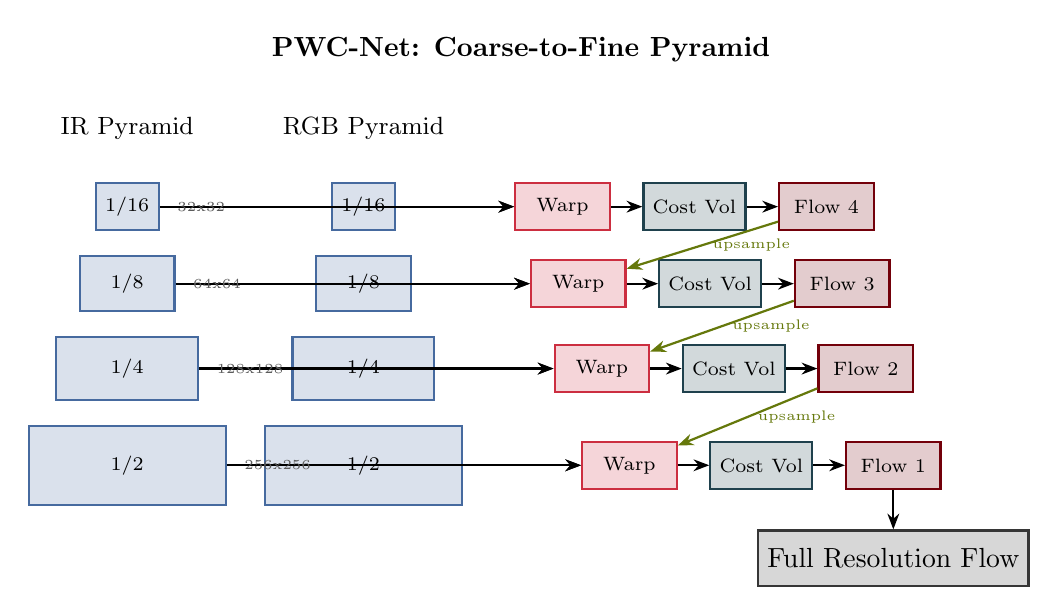
\begin{tikzpicture}[
    feat/.style={rectangle,draw=Atlantic,fill=Atlantic!20,thick,minimum width=1.5cm,minimum height=0.7cm,font=\scriptsize},
    warp/.style={rectangle,draw=Rose,fill=Rose!20,thick,minimum width=1.2cm,minimum height=0.6cm,font=\scriptsize},
    cost/.style={rectangle,draw=Congaree,fill=Congaree!20,thick,minimum width=1.2cm,minimum height=0.6cm,font=\scriptsize},
    flow/.style={rectangle,draw=Garnet,fill=Garnet!20,thick,minimum width=1.2cm,minimum height=0.6cm,font=\scriptsize},
    arrow/.style={-{Stealth[length=2mm]},thick}
]

\node[font=\bfseries] at (6,8.5) {PWC-Net: Coarse-to-Fine Pyramid};

% IR pyramid (left)
\node[font=\small] at (1,7.5) {IR Pyramid};
\node[feat,minimum width=0.8cm,minimum height=0.6cm] (ir-l4) at (1,6.5) {1/16};
\node[feat,minimum width=1.2cm,minimum height=0.7cm,below=0.3cm of ir-l4] (ir-l3) {1/8};
\node[feat,minimum width=1.8cm,minimum height=0.8cm,below=0.3cm of ir-l3] (ir-l2) {1/4};
\node[feat,minimum width=2.5cm,minimum height=1.0cm,below=0.3cm of ir-l2] (ir-l1) {1/2};

% RGB pyramid (right side)
\node[font=\small] at (4,7.5) {RGB Pyramid};
\node[feat,minimum width=0.8cm,minimum height=0.6cm] (rgb-l4) at (4,6.5) {1/16};
\node[feat,minimum width=1.2cm,minimum height=0.7cm,below=0.3cm of rgb-l4] (rgb-l3) {1/8};
\node[feat,minimum width=1.8cm,minimum height=0.8cm,below=0.3cm of rgb-l3] (rgb-l2) {1/4};
\node[feat,minimum width=2.5cm,minimum height=1.0cm,below=0.3cm of rgb-l2] (rgb-l1) {1/2};

% Level 4 processing (coarsest)
\node[warp,right=1.5cm of rgb-l4] (warp4) {Warp};
\node[cost,right=0.4cm of warp4] (cost4) {Cost Vol};
\node[flow,right=0.4cm of cost4] (flow4) {Flow 4};

\draw[arrow] (ir-l4) -- (warp4);
\draw[arrow] (rgb-l4) -- (warp4);
\draw[arrow] (warp4) -- (cost4);
\draw[arrow] (cost4) -- (flow4);

% Level 3
\node[warp,right=1.5cm of rgb-l3] (warp3) {Warp};
\node[cost,right=0.4cm of warp3] (cost3) {Cost Vol};
\node[flow,right=0.4cm of cost3] (flow3) {Flow 3};

\draw[arrow] (ir-l3) -- (warp3);
\draw[arrow] (rgb-l3) -- (warp3);
\draw[arrow] (warp3) -- (cost3);
\draw[arrow] (cost3) -- (flow3);
\draw[arrow,Horseshoe] (flow4) -- node[right,font=\tiny] {upsample} (warp3);

% Level 2
\node[warp,right=1.5cm of rgb-l2] (warp2) {Warp};
\node[cost,right=0.4cm of warp2] (cost2) {Cost Vol};
\node[flow,right=0.4cm of cost2] (flow2) {Flow 2};

\draw[arrow] (ir-l2) -- (warp2);
\draw[arrow] (rgb-l2) -- (warp2);
\draw[arrow] (warp2) -- (cost2);
\draw[arrow] (cost2) -- (flow2);
\draw[arrow,Horseshoe] (flow3) -- node[right,font=\tiny] {upsample} (warp2);

% Level 1 (finest)
\node[warp,right=1.5cm of rgb-l1] (warp1) {Warp};
\node[cost,right=0.4cm of warp1] (cost1) {Cost Vol};
\node[flow,right=0.4cm of cost1] (flow1) {Flow 1};

\draw[arrow] (ir-l1) -- (warp1);
\draw[arrow] (rgb-l1) -- (warp1);
\draw[arrow] (warp1) -- (cost1);
\draw[arrow] (cost1) -- (flow1);
\draw[arrow,Horseshoe] (flow2) -- node[right,font=\tiny] {upsample} (warp1);

% Final output
\node[rectangle,draw=Black90,fill=Black90!20,thick,minimum width=2cm,minimum height=0.7cm,below=0.5cm of flow1] (output) {Full Resolution Flow};
\draw[arrow] (flow1) -- (output);

% Annotations
\node[font=\tiny,Black70,right=0.1cm of ir-l4] {32x32};
\node[font=\tiny,Black70,right=0.1cm of ir-l3] {64x64};
\node[font=\tiny,Black70,right=0.1cm of ir-l2] {128x128};
\node[font=\tiny,Black70,right=0.1cm of ir-l1] {256x256};

\end{tikzpicture}
\end{document}
